%%%%%%%%%%%%%%%%%%%%%%%%%%%%%%%%%%%%%%%%%%%%%%%%%%%%%%%%%%%%%%%%%%%%%%%%%%%%%%%%%%
\begin{frame}[fragile]\frametitle{}
\begin{center}
{\Large Fine-tuning Using Hugging Face Transformers Library}
\end{center}
\end{frame}

%%%%%%%%%%%%%%%%%%%%%%%%%%%%%%%%%%%%%%%%%%%%%%%%%%%%%%%%%%%%%%%%%%%%%%%%%%%%%%%%%%
\begin{frame}[fragile]\frametitle{Introduction to Fine-Tuning}
  \begin{itemize}
    \item \textbf{Definition:} Process of training pre-existing models on smaller, domain-specific datasets to enhance task or domain performance.
    \item \textbf{Objective:} Refine capabilities and adapt models for specific applications.
    \item \textbf{Illustration with GPT-3:}
      \begin{itemize}
        \item GPT-3 designed for diverse NLP tasks but may lack optimization for specific domains.
        \item Example: Healthcare organization fine-tunes GPT-3 for generating patient reports, adapting to medical terminologies.
      \end{itemize}
    \item \textbf{Applicability Beyond LLMs:}
      \begin{itemize}
        \item Not exclusive to language models; applicable to various machine learning models.
        \item Example: Convolutional neural network fine-tuning for detecting trucks on highways.
      \end{itemize}
    \item \textbf{Key Principle:} Leverage pre-trained models, recalibrate parameters using novel data for new contexts or applications.
    \item \textbf{Considerations:} Beneficial when training data distribution significantly differs from specific application requirements.
  \end{itemize}
\end{frame}


%%%%%%%%%%%%%%%%%%%%%%%%%%%%%%%%%%%%%%%%%%%%%%%%%%%%%%%%%%%
\begin{frame}[fragile]\frametitle{What is a fine-tuned LLM?}


		\begin{center}
		\includegraphics[width=\linewidth,keepaspectratio]{rag8}
		\end{center}

{\tiny (Ref: Generative AI with Large Language Model - Abhinav  Kimothi)}

\end{frame}



%%%%%%%%%%%%%%%%%%%%%%%%%%%%%%%%%%%%%%%%%%%%%%%%%%%%%%%%%%%%%%%%%%%%%%%%%%%%%%%%%%
\begin{frame}[fragile]\frametitle{Why Fine-Tuning?}
  \begin{itemize}
    \item \textbf{General Models vs. Specialization:}
      \begin{itemize}
        \item Large language models designed for versatility, not task mastery.
        \item Fine-tuning essential for exceptional proficiency in specific tasks or domains.
      \end{itemize}
    \item \textbf{Versatility vs. Mastery:}
      \begin{itemize}
        \item Generic models proficient in multiple tasks but lack mastery.
        \item Fine-tuned models optimized for specific tasks, achieving mastery.
      \end{itemize}
    \item \textbf{Decision to Fine-Tune:}
      \begin{itemize}
        \item Driven by the need for superior performance in targeted applications.
        \item Highly effective specialists in designated areas.
      \end{itemize}
  \end{itemize}
\end{frame}


%%%%%%%%%%%%%%%%%%%%%%%%%%%%%%%%%%%%%%%%%%%%%%%%%%%%%%%%%%%%%%%%%%%%%%%%%%%%%%%%%%
\begin{frame}[fragile]\frametitle{Why Fine-Tuning?}
    \begin{itemize}
        \item Pre-trained models are trained and built with general-purpose tasks, with Fine-tuning we can improve the performance of pre-trained models in wide range of domain-specific tasks.
        \item Fine-tuning is a technique where a pre-trained model is trained on a new dataset.
		\item Fine Tuning has many approaches, one uses adjusting last layer with retraining on custom data, another has adopter auxiliary network which gets trained on custom data, some have full retraining with frozen earlier weights.
		\item Fine-tuning leverages a pre-trained model's knowledge and capabilities, saving significant time and resources compared to training a model from scratch. 
		\item Improve factual response by utilizing Domain-specific data. 
		\item Reduce Hallucinations.
    \end{itemize}
\end{frame}

%%%%%%%%%%%%%%%%%%%%%%%%%%%%%%%%%%%%%%%%%%%%%%%%%%%%%%%%%%%
\begin{frame}[fragile]\frametitle{What is a fine-tuned LLM?}

\begin{itemize}
  \item \textbf{Context Learning Limitation:}
    \begin{itemize}
      \item Through in-context learning or prompting, only a limited performance level is achievable.
    \end{itemize}

  \item \textbf{Challenges of Few-Shot Learning:}
    \begin{itemize}
      \item Few-shot learning may not be effective for smaller LLMs.
      \item Consumes significant space in the context window.
    \end{itemize}

  \item \textbf{Fine Tuning Overview:}
    \begin{itemize}
      \item Supervised learning process adjusting LLM weights.
      \item Uses a labeled dataset of prompt-completion pairs.
    \end{itemize}

  \item \textbf{Instruction Fine Tuning:}
    \begin{itemize}
      \item Trains LLM on examples of instructions and desired responses.
      \item Improves performance on instruction-specific tasks.
    \end{itemize}

  \item \textbf{Full Fine Tuning:}
    \begin{itemize}
      \item Updates all LLM parameters.
      \item Requires sufficient memory for storing and processing gradients and components.
    \end{itemize}
\end{itemize}


{\tiny (Ref: Generative AI with Large Language Model - Abhinav  Kimothi)}

\end{frame}


%%%%%%%%%%%%%%%%%%%%%%%%%%%%%%%%%%%%%%%%%%%%%%%%%%%%%%%%%%%%%%%%%%%%%%%%%%%%%%%%%%
\begin{frame}[fragile]\frametitle{Reasons for Fine-Tuning - Part 1}
  \begin{itemize}
    \item \textbf{Domain-Specific Adaptation:}
      \begin{itemize}
        \item Pre-trained LLMs not optimized for specific tasks or domains.
        \item Fine-tuning allows adaptation to nuances, enhancing performance.
        \item Example: Fine-tuning for document analysis in the legal domain.
      \end{itemize}
    \item \textbf{Shifts in Data Distribution:}
      \begin{itemize}
        \item Models may not generalize well to out-of-distribution examples.
        \item Fine-tuning aligns the model with new data distribution, improving performance.
        \item Example: Fine-tuning a sentiment analysis model for social media comments.
      \end{itemize}
    \item \textbf{Cost and Resource Efficiency:}
      \begin{itemize}
        \item Training from scratch requires a large dataset, fine-tuning is more efficient.
        \item Example: Adapting a pre-trained model for small e-commerce platform recommendations.
      \end{itemize}
  \end{itemize}
\end{frame}

%%%%%%%%%%%%%%%%%%%%%%%%%%%%%%%%%%%%%%%%%%%%%%%%%%%%%%%%%%%%%%%%%%%%%%%%%%%%%%%%%%
\begin{frame}[fragile]\frametitle{Reasons for Fine-Tuning - Part 2}
  \begin{itemize}
    \item \textbf{Out-of-Distribution Data Handling:}
      \begin{itemize}
        \item Fine-tuning mitigates suboptimal performance with modest dataset.
        \item Example: Fine-tuning a speech recognition model for a new regional accent.
      \end{itemize}
    \item \textbf{Knowledge Transfer:}
      \begin{itemize}
        \item Fine-tuning transfers general knowledge from pre-trained models to specific tasks.
        \item Example: Transferring medical knowledge to a healthcare chatbot.
      \end{itemize}
    \item \textbf{Task-Specific Optimization:}
      \begin{itemize}
        \item Fine-tuning optimizes model parameters for specific task objectives.
        \item Example: Optimizing a pre-trained model for code generation in software development.
      \end{itemize}
  \end{itemize}
\end{frame}


%%%%%%%%%%%%%%%%%%%%%%%%%%%%%%%%%%%%%%%%%%%%%%%%%%%%%%%%%%%%%%%%%%%%%%%%%%%%%%%%%%
\begin{frame}[fragile]\frametitle{Reasons for Fine-Tuning - Part 3}
  \begin{itemize}
    \item \textbf{Adaptation to User Preferences:}
      \begin{itemize}
        \item Fine-tuning aligns the model with user preferences and task requirements.
        \item Example: Fine-tuning a virtual assistant model for user-specific language and tone.
      \end{itemize}
    \item \textbf{Continual Learning:}
      \begin{itemize}
        \item Fine-tuning supports continual learning, adapting to evolving data and user needs.
        \item Example: Continually updating a news summarization model for evolving news topics.
      \end{itemize}
  \end{itemize}
\end{frame}

%%%%%%%%%%%%%%%%%%%%%%%%%%%%%%%%%%%%%%%%%%%%%%%%%%%%%%%%%%%%%%%%%%%%%%%%%%%%%%%%%%
\begin{frame}[fragile]\frametitle{Challenges and Solutions: In-Context Learning}
    \begin{itemize}
        \item Prominent technique for task-specific adaptation.
        \item Challenges include limited context window and real-time optimization.
        \item Context window restricts processing of long sequences.
        \item Real-time optimization is difficult during progression through the context window.
    \end{itemize}
\end{frame}

%%%%%%%%%%%%%%%%%%%%%%%%%%%%%%%%%%%%%%%%%%%%%%%%%%%%%%%%%%%%%%%%%%%%%%%%%%%%%%%%%%
\begin{frame}[fragile]\frametitle{Challenges with Few-Shot Learning}
    \begin{itemize}
        \item Effective for larger LLMs, less so for smaller models.
        \item Smaller models struggle to learn complex patterns from few examples.
        \item Few-shot learning demands a large context window.
        \item Resource-intensive and impractical for memory-constrained environments.
    \end{itemize}
\end{frame}

%%%%%%%%%%%%%%%%%%%%%%%%%%%%%%%%%%%%%%%%%%%%%%%%%%%%%%%%%%%
\begin{frame}[fragile]\frametitle{Ways to fine-tune}


		\begin{center}
		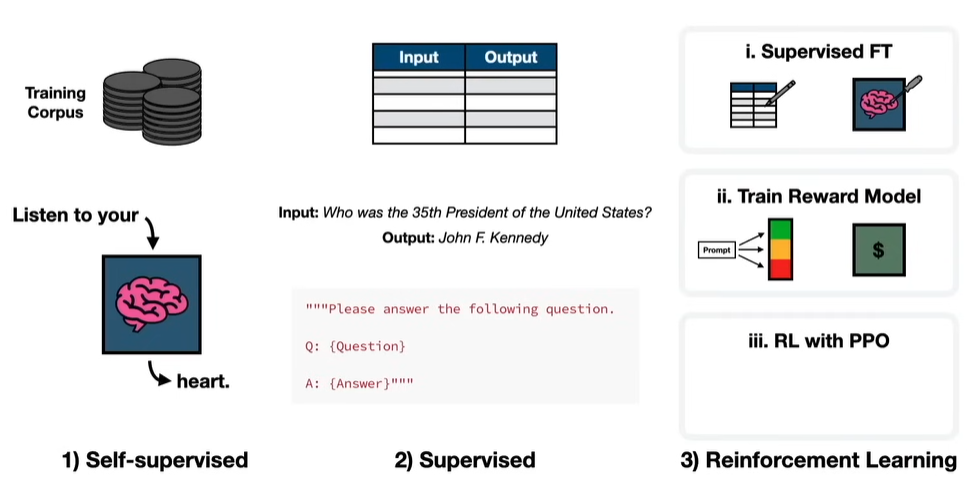
\includegraphics[width=\linewidth,keepaspectratio]{finetune7}
		\end{center}

{\tiny (Ref: Fine-tuning Large Language Models (LLMs) | w/ Example Code - Shaw Talebi)}

\end{frame}

%%%%%%%%%%%%%%%%%%%%%%%%%%%%%%%%%%%%%%%%%%%%%%%%%%%%%%%%%%%
\begin{frame}[fragile]\frametitle{Ways to change parameters/weights}


		\begin{center}
		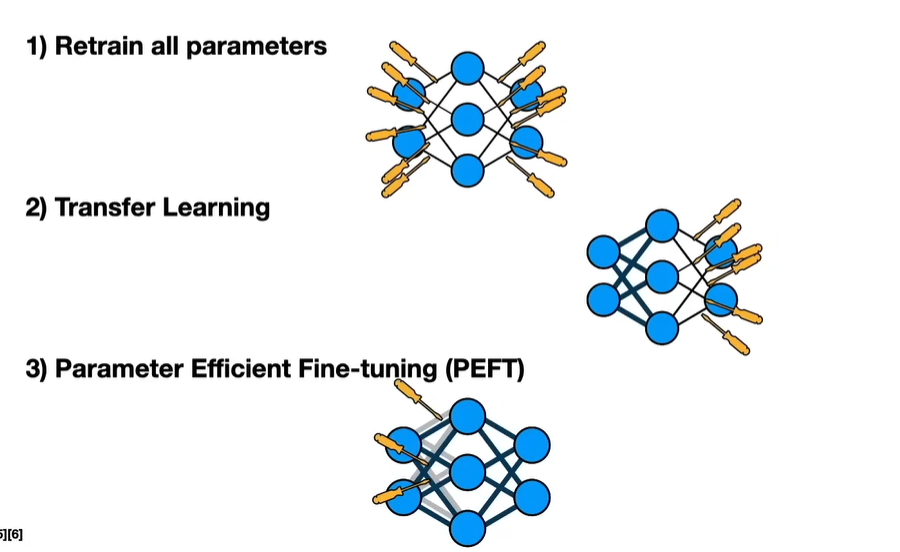
\includegraphics[width=\linewidth,keepaspectratio]{finetune8}
		\end{center}

{\tiny (Ref: Fine-tuning Large Language Models (LLMs) | w/ Example Code - Shaw Talebi)}

\end{frame}


%%%%%%%%%%%%%%%%%%%%%%%%%%%%%%%%%%%%%%%%%%%%%%%%%%%%%%%%%%%%%%%%%%%%%%%%%%%%%%%%%%
\begin{frame}[fragile]\frametitle{Understanding Fine-Tuning}
    \begin{itemize}
        \item Widely used for customizing pre-trained LLMs to specific tasks.
        \item Involves training on labeled prompt-completion pairs.
        \item Allows model to adjust weights for task alignment.
    \end{itemize}
\end{frame}

%%%%%%%%%%%%%%%%%%%%%%%%%%%%%%%%%%%%%%%%%%%%%%%%%%%%%%%%%%%%%%%%%%%%%%%%%%%%%%%%%%
\begin{frame}[fragile]\frametitle{Unsupervised Fine-Tuning Methods}

\begin{itemize}
\item \textbf{Unsupervised Full Fine-Tuning:}
  \begin{itemize}
	\item Relevant for updating LLM knowledge base without changing existing behavior.
	\item Example: Fine-tuning on legal literature or adapting to a new language using unstructured datasets.
  \end{itemize}
\item \textbf{Contrastive Learning:}
  \begin{itemize}
	\item Trains the model to discern between similar and dissimilar examples in the latent space.
	\item Beneficial for tasks requiring nuanced understanding of similarities and distinctions.
  \end{itemize}
\end{itemize}
\end{frame}

%%%%%%%%%%%%%%%%%%%%%%%%%%%%%%%%%%%%%%%%%%%%%%%%%%%%%%%%%%%%%%%%%%%%%%%%%%%%%%%%%%
\begin{frame}[fragile]\frametitle{Supervised Fine-Tuning Methods}

\begin{itemize}
\item \textbf{Parameter-Efficient Fine-Tuning (PEFT):}
  \begin{itemize}
	\item Aims to reduce computational expenses by selectively updating a small set of parameters.
	\item Example: Low-rank adaptation (LoRA) technique focuses on updating only relevant parameters.
  \end{itemize}
\item \textbf{Supervised Full Fine-Tuning:}
  \begin{itemize}
	\item Involves updating all parameters of the language model during training.
	\item Resource-intensive but ensures thorough adaptation of the entire model to the task or domain.
  \end{itemize}
\item \textbf{Instruction Fine-Tuning:}
  \begin{itemize}
	\item Involves training the model using examples with explicit instructions for specific queries or tasks.
	\item Suitable for applications where precise task execution is essential.
  \end{itemize}
\item \textbf{Reinforcement Learning from Human Feedback (RLHF):}
  \begin{itemize}
	\item Incorporates reinforcement learning principles with human evaluators providing ratings.
	\item Ratings serve as rewards, guiding the model to optimize parameters based on human preferences.
  \end{itemize}
\end{itemize}

\end{frame}

%%%%%%%%%%%%%%%%%%%%%%%%%%%%%%%%%%%%%%%%%%%%%%%%%%%%%%%%%%%%%%%%%%%%%%%%%%%%%%%%%%
\begin{frame}[fragile]\frametitle{Instruction Fine-Tuning}
  \begin{itemize}
    \item \textbf{Overview:}
      \begin{itemize}
        \item Instruction fine-tuning enhances LLMs for real-world applications.
        \item Differs from standard supervised fine-tuning by augmenting examples with explicit instructions.
        \item Instruction-tuned models generalize effectively to new tasks, providing additional context.
      \end{itemize}
    \item \textbf{Value in NLP and ML:}
      \begin{itemize}
        \item Instruction fine-tuning is crucial in the evolving landscape of NLP and ML.
        \item Enables LLMs to adapt to specific tasks with nuanced instructions.
      \end{itemize}	  
  \end{itemize}

\begin{center}
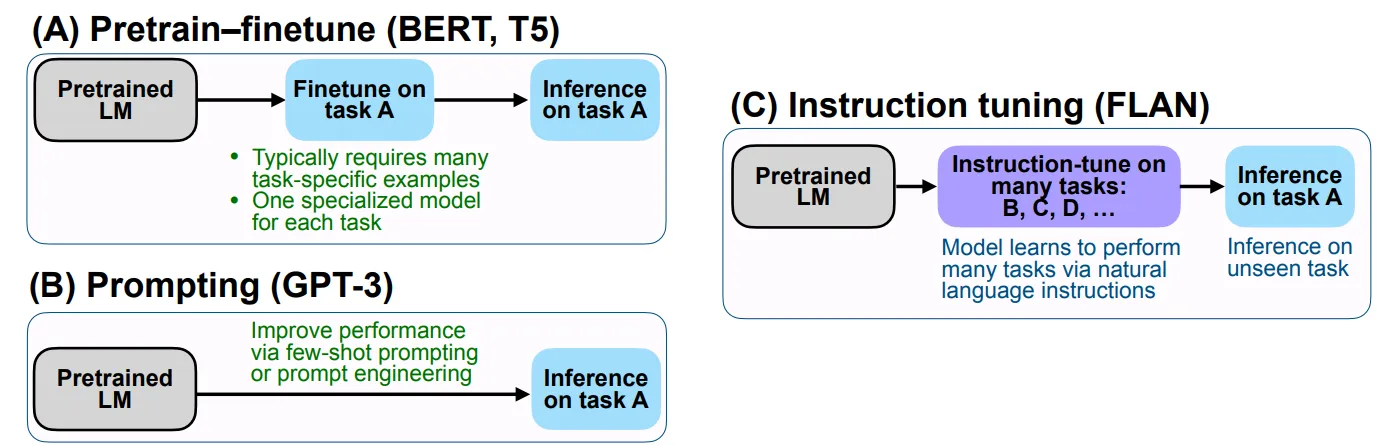
\includegraphics[width=\linewidth,keepaspectratio]{llm128}
\end{center}				

{\tiny (Ref: Applied LLMs Mastery 2024 - Aishwarya Reganti)}

\end{frame}


%%%%%%%%%%%%%%%%%%%%%%%%%%%%%%%%%%%%%%%%%%%%%%%%%%%%%%%%%%%%%%%%%%%%%%%%%%%%%%%%%%
\begin{frame}[fragile]\frametitle{Natural Instructions Dataset}
  \begin{itemize}
    \item \textbf{Dataset Overview:}
      \begin{itemize}
        \item "Natural Instructions" dataset consists of 193,000 instruction-output examples.
        \item Sourced from 61 existing English NLP tasks.
        \item Structured approach with crowd-sourced instructions aligned to a common schema.
      \end{itemize}
    \item \textbf{Unique Features:}
      \begin{itemize}
        \item Each instruction associated with a task, providing explicit guidance for the model.
        \item Covers fields like definition, things to avoid, positive and negative examples.
        \item Structured nature makes it valuable for fine-tuning, offering clear and detailed instructions.
      \end{itemize}
  \end{itemize}
\end{frame}


%%%%%%%%%%%%%%%%%%%%%%%%%%%%%%%%%%%%%%%%%%%%%%%%%%%%%%%%%%%%%%%%%%%%%%%%%%%%%%%%%%
\begin{frame}[fragile]\frametitle{Natural Instructions Example}

\begin{center}
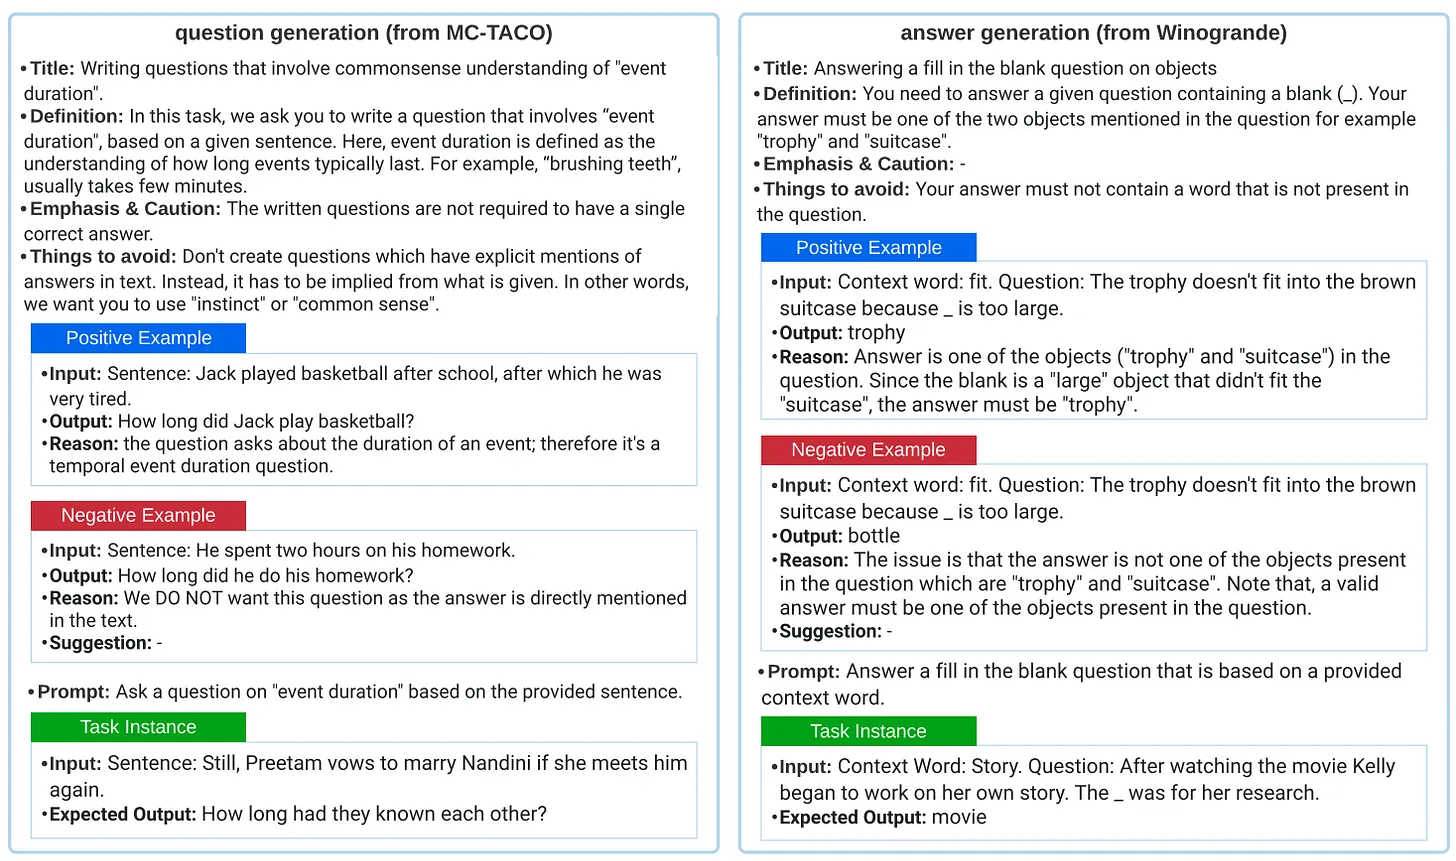
\includegraphics[width=\linewidth,keepaspectratio]{llm129}
\end{center}				

{\tiny (Ref: Applied LLMs Mastery 2024 - Aishwarya Reganti)}

\end{frame}

%%%%%%%%%%%%%%%%%%%%%%%%%%%%%%%%%%%%%%%%%%%%%%%%%%%%%%%%%%%%%%%%%%%%%%%%%%%%%%%%%%
\begin{frame}[fragile]\frametitle{Leveraging Instruction Fine-Tuning}
    \begin{itemize}
        \item Extension of traditional fine-tuning.
        \item Trains model on examples of instructions and desired responses.
        \item Offers improved interpretability, controlled outputs, and reduced biases.
        \item Enables explicit task specification learning for enhanced performance.
    \end{itemize}
\end{frame}

%%%%%%%%%%%%%%%%%%%%%%%%%%%%%%%%%%%%%%%%%%%%%%%%%%%%%%%%%%%%%%%%%%%%%%%%%%%%%%%%%%
\begin{frame}[fragile]\frametitle{Full Fine-Tuning Potential}
    \begin{itemize}
        \item Updates all parameters of the language model during training.
        \item Enhances adaptability to specific tasks for potentially better performance.
        \item Demands significant memory for processing gradients and other components.
        \item Challenging to implement on resource-constrained devices or environments.
    \end{itemize}
\end{frame}

%%%%%%%%%%%%%%%%%%%%%%%%%%%%%%%%%%%%%%%%%%%%%%%%%%%%%%%%%%%%%%%%%%%%%%%%%%%%%%%%%%
\begin{frame}[fragile]\frametitle{Reinforcement Learning from Human Feedback (RLHF)}
  \begin{itemize}
    \item \textbf{Overview:}
      \begin{itemize}
        \item RLHF enhances language models by incorporating human feedback.
        \item Aims to align models more closely with intricate human values.
      \end{itemize}
  \end{itemize}
  
\begin{center}
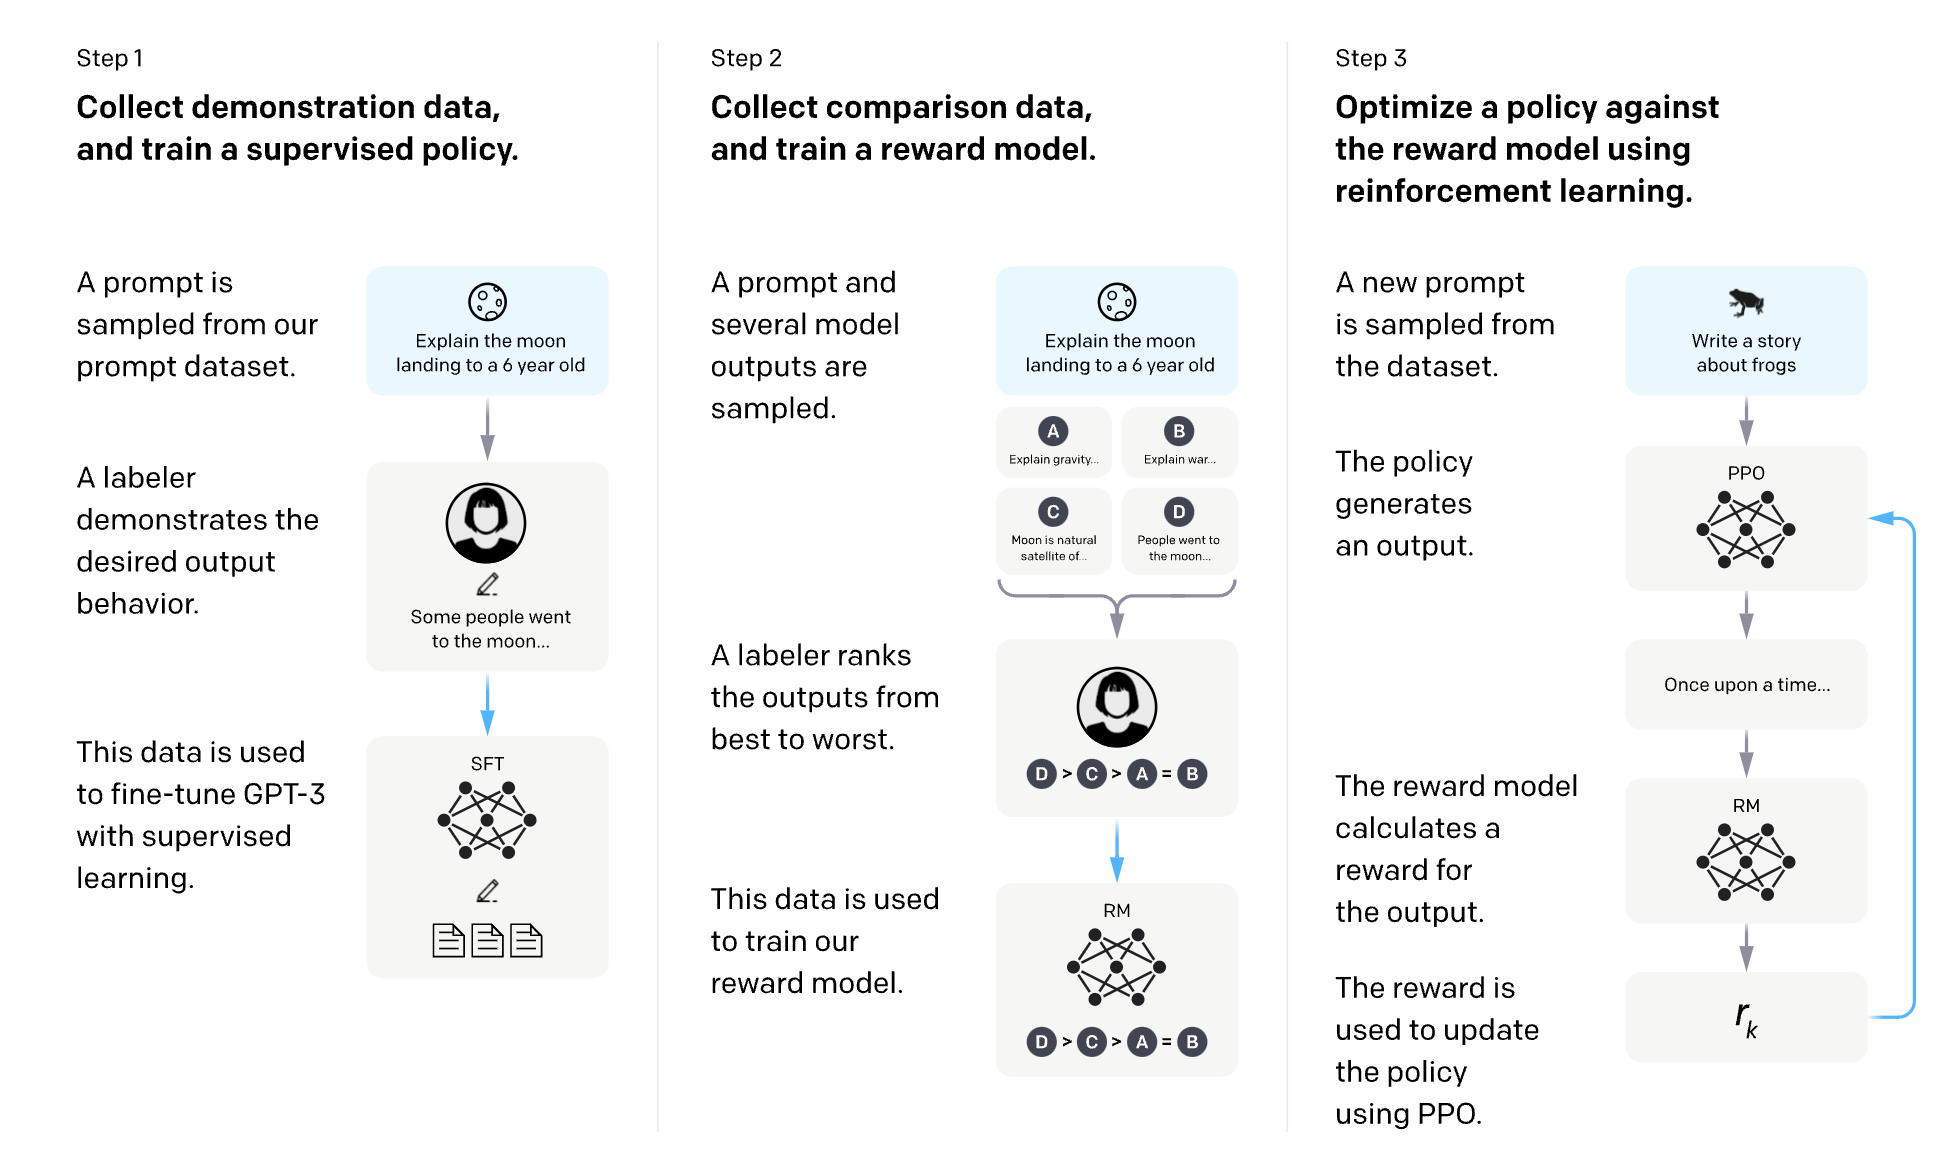
\includegraphics[width=0.8\linewidth,keepaspectratio]{llm130}
\end{center}				

{\tiny (Ref: Applied LLMs Mastery 2024 - Aishwarya Reganti)}  
\end{frame}

%%%%%%%%%%%%%%%%%%%%%%%%%%%%%%%%%%%%%%%%%%%%%%%%%%%%%%%%%%%%%%%%%%%%%%%%%%%%%%%%%%
\begin{frame}[fragile]\frametitle{RLHF Process - Step 1}
  \begin{itemize}
    \item \textbf{Pretraining Language Models (LMs):}
      \begin{itemize}
        \item RLHF starts with a pretrained LM, typically achieved through classical pretraining objectives.
        \item Initial LM, flexible in size, can undergo optional fine-tuning on additional data.
        \item Crucial to have a model with positive response to diverse instructions.
      \end{itemize}
  \end{itemize}
\end{frame}

%%%%%%%%%%%%%%%%%%%%%%%%%%%%%%%%%%%%%%%%%%%%%%%%%%%%%%%%%%%%%%%%%%%%%%%%%%%%%%%%%%
\begin{frame}[fragile]\frametitle{RLHF Process - Step 2}
  \begin{itemize}
    \item \textbf{Reward Model Training:}
      \begin{itemize}
        \item Involves generating a reward model (RM) calibrated with human preferences.
        \item RM assigns scalar rewards to text sequences, reflecting human preferences.
        \item Dataset for training RM generated by sampling prompts, passing through initial LM, and ranking by human annotators.
        \item Reward function combines preference model and a penalty on RL policy vs. initial model difference.
      \end{itemize}
  \end{itemize}
\end{frame}

%%%%%%%%%%%%%%%%%%%%%%%%%%%%%%%%%%%%%%%%%%%%%%%%%%%%%%%%%%%%%%%%%%%%%%%%%%%%%%%%%%
\begin{frame}[fragile]\frametitle{RLHF Process - Step 3}
  \begin{itemize}
    \item \textbf{Fine-Tuning with RL:}
      \begin{itemize}
        \item Final step involves fine-tuning the initial LLM using reinforcement learning.
        \item Proximal Policy Optimization (PPO) commonly used for RL algorithm.
        \item RL policy is LM that takes prompt, produces text, with actions corresponding to tokens in LM's vocabulary.
        \item PPO updates LM's parameters to maximize reward metrics, aligning model with human preferences.
        \item Some parameters frozen due to computational constraints.
      \end{itemize}
  \end{itemize}
\end{frame}

%%%%%%%%%%%%%%%%%%%%%%%%%%%%%%%%%%%%%%%%%%%%%%%%%%%%%%%%%%%%%%%%%%%%%%%%%%%%%%%%%%
\begin{frame}[fragile]\frametitle{Direct Preference Optimization (DPO)}
  \begin{itemize}
    \item \textbf{Overview:}
      \begin{itemize}
        \item DPO is equivalent to RLHF and gaining significant traction.
        \item Offers a straightforward method for fine-tuning large language models based on human preferences.
        \item Eliminates the need for a complex reward model, directly incorporating user feedback into the optimization process.
      \end{itemize}
    \item \textbf{User-Friendly Approach:}
      \begin{itemize}
        \item Users compare two model-generated outputs and express preferences.
        \item LLM adjusts its behavior accordingly, simplifying the optimization process.
        \item Advantages include ease of implementation, computational efficiency, and greater control over LLM's behavior.
      \end{itemize}
  \end{itemize}

\begin{center}
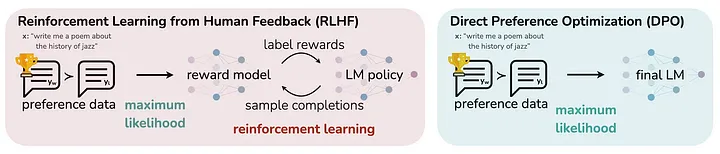
\includegraphics[width=\linewidth,keepaspectratio]{llm131}
\end{center}				

{\tiny (Ref: Applied LLMs Mastery 2024 - Aishwarya Reganti)}

\end{frame}


%%%%%%%%%%%%%%%%%%%%%%%%%%%%%%%%%%%%%%%%%%%%%%%%%%%%%%%%%%%%%%%%%%%%%%%%%%%%%%%%%%
\begin{frame}[fragile]\frametitle{Comparison: DPO vs RLHF}
  \begin{itemize}
    \item \textbf{DPO Approach:}
      \begin{itemize}
        \item Directly optimizes LM based on user preferences without a separate reward model.
        \item Users compare two model-generated outputs to guide the optimization process.
      \end{itemize}

    \item \textbf{Maximum Likelihood in LLM Training:}
      \begin{itemize}
        \item Maximum likelihood is a principle used during LLM training.
        \item Involves adjusting model's parameters to maximize the likelihood of generating actual sequences observed in training data.
        \item Helps LLM learn to generate text similar to examples it was trained on.
      \end{itemize}
    \item \textbf{RLHF Approach:}
      \begin{itemize}
        \item Follows a more structured path, leveraging reinforcement learning principles.
        \item Involves training a reward model to identify and reward desirable LM outputs.
        \item Reward model guides LM's training process, shaping its behavior towards positive outcomes.
      \end{itemize}
    \item \textbf{DPO - A Simpler Approach:}
      \begin{itemize}
        \item Direct Policy Optimization (DPO) takes a straightforward path.
        \item Sidesteps the need for a complex reward model in fine-tuning Large Language Models (LLMs).
        \item Optimizes LLM directly based on user preferences by comparing two outputs.
      \end{itemize}
  \end{itemize}
\end{frame}

%%%%%%%%%%%%%%%%%%%%%%%%%%%%%%%%%%%%%%%%%%%%%%%%%%%%%%%%%%%%%%%%%%%%%%%%%%%%%%%%%%
\begin{frame}[fragile]\frametitle{DPO Advantages}
  \begin{itemize}
    \item \textbf{Ease of Implementation:}
      \begin{itemize}
        \item DPO is more user-friendly, eliminating the need for a separate reward model.
        \item Accessible to a broader audience due to its simplicity.
      \end{itemize}
    \item \textbf{Computational Efficiency:}
      \begin{itemize}
        \item Operates directly on the LLM, leading to faster training times.
        \item Lower computational costs compared to RLHF.
      \end{itemize}
    \item \textbf{Greater Control:}
      \begin{itemize}
        \item Users have direct control over LLM's behavior without complexities.
        \item Enables guidance toward specific goals and preferences.
      \end{itemize}
    \item \textbf{Faster Convergence:}
      \begin{itemize}
        \item Due to its simpler structure and direct optimization, DPO often achieves faster results.
        \item Suitable for tasks with rapid iteration needs.
      \end{itemize}
    \item \textbf{Improved Performance:}
      \begin{itemize}
        \item Recent research suggests DPO can outperform RLHF in sentiment control and response quality.
        \item Particularly effective in summarization and dialogue tasks.
      \end{itemize}
  \end{itemize}
\end{frame}

%%%%%%%%%%%%%%%%%%%%%%%%%%%%%%%%%%%%%%%%%%%%%%%%%%%%%%%%%%%%%%%%%%%%%%%%%%%%%%%%%%
\begin{frame}[fragile]\frametitle{RLHF - A More Structured Approach}
  \begin{itemize}
    \item \textbf{More Structured Path:}
      \begin{itemize}
        \item Reinforcement Learning from Human Feedback (RLHF) follows a more structured path.
        \item Leverages reinforcement learning principles in three training phases.
      \end{itemize}
    \item \textbf{Complexity:}
      \begin{itemize}
        \item RLHF can be more complex and sometimes unstable.
        \item Demands more computational resources and deals with convergence, drift, or uncorrelated distribution problems.
      \end{itemize}
    \item \textbf{Flexibility in Defining Rewards:}
      \begin{itemize}
        \item RLHF allows more nuanced reward structures, beneficial for precise control over LLM's output.
      \end{itemize}
    \item \textbf{Handling Diverse Feedback Formats:}
      \begin{itemize}
        \item RLHF can handle various forms of human feedback, including numerical ratings or textual corrections.
        \item DPO primarily relies on binary preferences for user feedback.
      \end{itemize}
    \item \textbf{Handling Large Datasets:}
      \begin{itemize}
        \item RLHF can be more efficient in handling massive datasets, especially with distributed training techniques.
      \end{itemize}
  \end{itemize}
\end{frame}

%%%%%%%%%%%%%%%%%%%%%%%%%%%%%%%%%%%%%%%%%%%%%%%%%%%%%%%%%%%%%%%%%%%%%%%%%%%%%%%%%%
\begin{frame}[fragile]\frametitle{Summary}
  \begin{itemize}
    \item \textbf{Choice Depends On:}
      \begin{itemize}
        \item Specific task requirements.
        \item Available computational resources.
        \item Desired level of control over LLM's behavior.
      \end{itemize}
    \item \textbf{Strengths and Weaknesses:}
      \begin{itemize}
        \item Both methods offer strengths and weaknesses in different contexts.
        \item Evolving and enhancing fine-tuning processes for LLMs.
      \end{itemize}
  \end{itemize}
\end{frame}


%%%%%%%%%%%%%%%%%%%%%%%%%%%%%%%%%%%%%%%%%%%%%%%%%%%%%%%%%%%
\begin{frame}[fragile]\frametitle{What is Parameter Efficient Fine Tuning?}

\begin{itemize}
  \item \textbf{Full Fine Tuning:}
    \begin{itemize}
      \item Requires memory for the entire model, optimizers, gradients, etc.
      \item Similar memory demands as pre-training.
    \end{itemize}

  \item \textbf{Parameter-Efficient Fine Tuning (PEFT):}
    \begin{itemize}
      \item Fine-tunes only a subset of model parameters.
      \item In some cases, leaves the original weights untouched.
    \end{itemize}
\end{itemize}


{\tiny (Ref: Generative AI with Large Language Model - Abhinav  Kimothi)}

\end{frame}


%%%%%%%%%%%%%%%%%%%%%%%%%%%%%%%%%%%%%%%%%%%%%%%%%%%%%%%%%%%
\begin{frame}[fragile]\frametitle{What is Parameter Efficient Fine Tuning?}


		\begin{center}
		\includegraphics[width=\linewidth,keepaspectratio]{rag9}
		\end{center}

{\tiny (Ref: Generative AI with Large Language Model - Abhinav  Kimothi)}

\end{frame}

%%%%%%%%%%%%%%%%%%%%%%%%%%%%%%%%%%%%%%%%%%%%%%%%%%%%%%%%%%%%%%%%%%%%%%%%%%%%%%%%%%
\begin{frame}[fragile]\frametitle{Parameter Efficient Fine-Tuning (PEFT)}
  \begin{itemize}
    \item \textbf{Addressing Resource Intensity:}
      \begin{itemize}
        \item PEFT addresses the resource-intensive nature of fine-tuning Large Language Models (LLMs).
        \item Full fine-tuning modifies all parameters, while PEFT fine-tunes only a small subset, minimizing computational demands.
      \end{itemize}
  \end{itemize}
\end{frame}

%%%%%%%%%%%%%%%%%%%%%%%%%%%%%%%%%%%%%%%%%%%%%%%%%%%%%%%%%%%%%%%%%%%%%%%%%%%%%%%%%%
\begin{frame}[fragile]\frametitle{Advantages of PEFT}
  \begin{itemize}
    \item \textbf{Computational Efficiency:}
      \begin{itemize}
        \item PEFT fine-tunes LLMs with significantly fewer parameters than full fine-tuning.
        \item Feasible on less powerful hardware or in resource-constrained environments.
      \end{itemize}
    \item \textbf{Memory Efficiency:}
      \begin{itemize}
        \item Freezing pretrained model weights minimizes excessive memory usage.
        \item Suitable for tasks with memory constraints.
      \end{itemize}
    \item \textbf{Catastrophic Forgetting Mitigation:}
      \begin{itemize}
        \item PEFT prevents catastrophic forgetting observed in full fine-tuning.
        \item Ensures retention of valuable information during adaptation to new tasks.
      \end{itemize}
    \item \textbf{Versatility Across Modalities:}
      \begin{itemize}
        \item PEFT is effective in various modalities such as computer vision and audio.
        \item Applicable to a wide range of downstream tasks beyond natural language processing.
      \end{itemize}
  \end{itemize}
\end{frame}

%%%%%%%%%%%%%%%%%%%%%%%%%%%%%%%%%%%%%%%%%%%%%%%%%%%%%%%%%%%%%%%%%%%%%%%%%%%%%%%%%%
\begin{frame}[fragile]\frametitle{Advantages of PEFT (Contd.)}
  \begin{itemize}
    \item \textbf{Modular Adaptation for Multiple Tasks:}
      \begin{itemize}
        \item PEFT's modular nature allows the same pretrained model to be adapted for multiple tasks.
        \item Small task-specific weights are added, avoiding the need for full copies for different applications.
      \end{itemize}
    \item \textbf{INT8 Tuning:}
      \begin{itemize}
        \item PEFT includes INT8 (8-bit integer) tuning, showcasing adaptability to different quantization techniques.
        \item Enables fine-tuning even on platforms with limited computational resources.
      \end{itemize}
  \end{itemize}
\end{frame}

%%%%%%%%%%%%%%%%%%%%%%%%%%%%%%%%%%%%%%%%%%%%%%%%%%%%%%%%%%%%%%%%%%%%%%%%%%%%%%%%%%
\begin{frame}[fragile]\frametitle{Summary of PEFT}
  \begin{itemize}
    \item PEFT offers a \textbf{practical and efficient solution} for fine-tuning large language models.
    \item Addresses \textbf{computational and memory challenges} while maintaining performance on downstream tasks.
  \end{itemize}
\end{frame}

%%%%%%%%%%%%%%%%%%%%%%%%%%%%%%%%%%%%%%%%%%%%%%%%%%%%%%%%%%%
\begin{frame}[fragile]{Limitations of Fine-Tuning}
    \begin{itemize}
        \item Catastrophic Forgetting: Fine-tuned models may forget some aspects of their pre-trained knowledge as they adapt to the new task.
        \item Computational requirements: Fine Tuning LLMs requires A100 GPU support.
        \item Full Fine-Tuning learning parameter dimensions is equal to the pre-trained learning parameters
    \end{itemize}
\end{frame}

